\documentclass[11pt]{article}
\usepackage{setspace}

\usepackage[margin=1in]{geometry}


\usepackage{rawfonts}
\usepackage{natbib}
\bibliographystyle{abbrvnat}
\usepackage{hyperref}
\usepackage{tkz-euclide}
\usepackage{pgfplots}

 \usetkzobj{all}
 
 \usepackage{amssymb,amsmath,amsthm}

\usepackage{makecell}

\renewcommand\theadalign{bc}
\renewcommand\theadfont{\bfseries}
\renewcommand\theadgape{\Gape[4pt]}
\renewcommand\cellgape{\Gape[4pt]}

\renewcommand\floatpagefraction{.9}
\renewcommand\topfraction{.9}
\renewcommand\bottomfraction{.9}
\renewcommand\textfraction{.1}   
\setcounter{totalnumber}{50}
\setcounter{topnumber}{50}
\setcounter{bottomnumber}{50}


\onehalfspacing
\setlength{\bibsep}{0pt plus 0.3ex}

\newcommand{\grad}{\nabla} % for gradient


\newtheorem{theorem}{Theorem}

\hyphenation{USGBC}


% Definitions of handy macros can go here

\newcommand{\LEED}{\textsc{LEED} }

\newcommand{\One}{\mathfrak{1}}
\newcommand{\dataset}{{\cal D}}
\newcommand{\fracpartial}[2]{\frac{\partial #1}{\partial  #2}}
\renewcommand{\vec}[1]{\mathbf{ #1 }}

\usepackage{enumitem}
%\setlist{nosep} % or \setlist{noitemsep} to leave space around whole list
% Short headings should be running head and authors last names

\newtheorem{defn}{Definition}


\usepackage{amsmath,mleftright}
\usepackage{xparse}

\NewDocumentCommand{\evalat}{sO{\big}mm}{%
  \IfBooleanTF{#1}
   {\mleft. #3 \mright|_{#4}}
   {#3#2|_{#4}}%
}


\begin{document}

\title{New Invariants for Automated Market Making}

\author{Abraham Othman \\
        The Wharton School, University of Pennsylvania\\
       \texttt{abrahamo@wharton.upenn.edu}}

\maketitle

\begin{abstract}%   <- trailing '%' for backward compatibility of .sty file
Automated market makers rely on invariants to price transactions with participants in distributed exchanges. We introduce a new family of invariants derived from the solutions to a  simple, parameterized partial differential equation. Our family spans from existing constant-product market makers which do not rely on priors to fixed-price market makers which rely exclusively on priors.
\end{abstract}


\section{Introduction}
Imagine a sportsbook taking bets on a football game where one of the teams has a large following of interested supporters. How should the sportsbook operator set their estimate of the game's outcome? Setting the \emph{a priori} objectively correct estimate would tend to lead to too many bets on the popular team, and therefore expose the sportsbook to large losses if the popular team wins. On the other hand, setting a line that is heavily skewed against the popular team in order to try and balance the market maker's exposure to the outcome is likely to lead to limited betting, which ultimately implies limited profitability. A market maker---which is what the sportsbook is in this context---has a complex role because of the need to balance the competing demands of inventory and expected value. Intuitively, the correct answer is not to naively optimize for expected gain, nor to avoid all potential loss, but rather to carve out an intermediate solution that balances these competing aims.

One solution to the sportsbook problem is to operate an online exchange in an order book model, where various bettors can post their own bids and offers on the teams, with the sportsbook taking a cut of transactions or winnings. However, operating an order book is not practicable in typical decentralized finance settings because the Ethereum gas fees associated with posting, matching, and withdrawing exchange orders are too high for viability.

Consequently, transactions in the latest generation of Decentralized Exchanges (DEXs) are typically mediated through \emph{automated market makers} built-in to their non-custodial smart contracts. Automated market makers are mathematical formulas that systematize the behavior of the human market makers that exist in financial, betting, and prediction markets. 

The defining feature for an automated market maker in a DEX is the market maker's \emph{invariant} function, a mapping from its holdings to a single scalar value, which is used to rationalize its interactions with market participants. The market maker maintains fair pricing for atomic swap trades by maintaining the level of its invariant. On the other hand, a liquidity provider adding or removing liquidity results in changes to the level of the invariant. Figure~\ref{fig:twoasset} is a graphical depiction of the relationship between the invariant function and participant actions in a simple two-asset case.

\begin{figure}[htbp]
\begin{center}
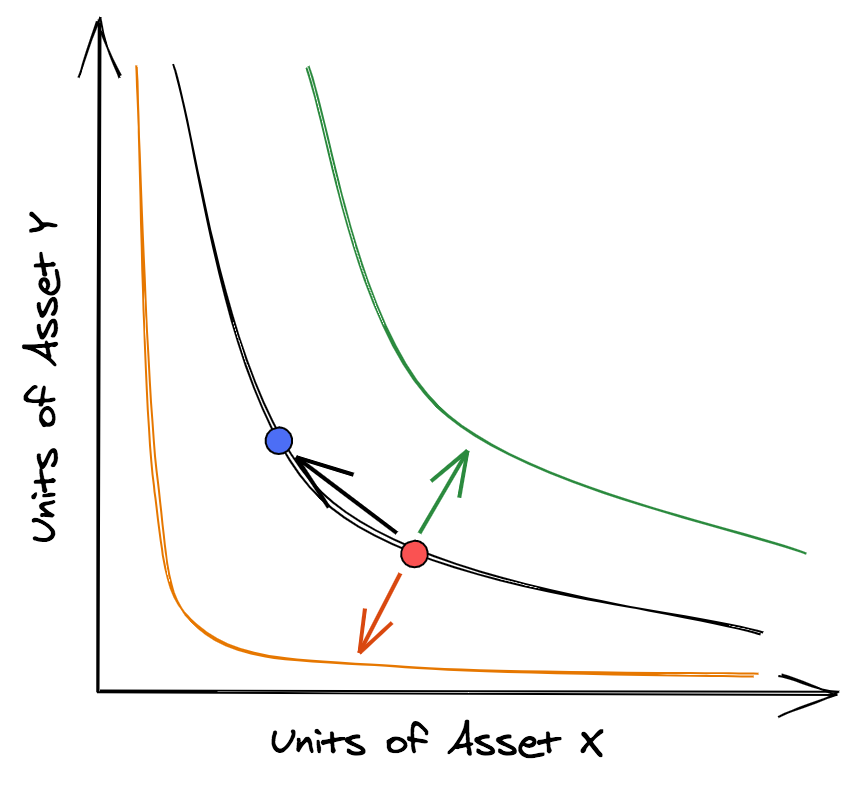
\includegraphics[width=0.5\textwidth]{TwoAssets}
\caption{Graphical depiction of a simple two-asset market, with the market maker's liquidity in each asset depicted along its respective axis. The automated market maker currently holds the position denoted by the red circle. The black curve is the level set of the invariant at the current asset level. The black arrow represents a swap transaction. Observe that the swap involves the trader adding the Y asset liquidity and removing X asset liquidity, but that the market maker's invariant stays at a constant value.
The green arrow represents moving the automated market maker to a higher invariant value through adding liquidity. The green curve is the level set of that higher invariant value. The orange arrow represents moving the automated market maker to a lower invariant value through removing liquidity. The orange curve is the level set of that lower invariant value.
}
\label{fig:twoasset}
\end{center}
\end{figure}

In this paper, we develop a family of automated market maker invariants that span between the two existing extremes of market making that are currently popular in DEXs: a fixed-price market maker that {only} relies on prior values, and the constant-product market maker that {only} relies on the market maker's inventory (the latter is used by the popular Uniswap DEX). Our intermediate invariant functions balance, to varying degrees, the market maker's competing demands of profitability and risk aversion.

 %We show that an intermediate invariant function---one that balances the competing constraints of  in-between these two extremes has a particularly attractive and simple functional form. 

Throughout this study we ignore an important aspect of automated market making: the fees charged to traders that would be used to subsidize liquidity providers. In practice with our invariants trading fees would be added as a separate fee independent from the slippage associated with the risk of a market maker's asset holdings (as in~\citet{Othman12:Profit}). 
%
This design is distinct from an alternative stream of automated market maker research where trading fees are incorporated implicitly within the market maker's risk response, as in the liquidity-sensitive design of~\citet{Othman13:OPRS}.

\section{Exposition}

The automated market maker has holdings of $n$ assets. We denote the nominal amount of those assets held by the market maker as a vector in the positive orthant $\Re_+^n \equiv \{\vec{x}\ |\ x_i \geq 0 \}$.

Without loss of generality we take the first asset as our numeraire and express fair-market prices $\vec{p}$ relative to that first asset, so that $p_1 = 1$, $M_1=1$, and $p_{i \neq 1} = 1/M_i$. These fair-market prices are the market maker's \emph{prior}, and can be set from external sources or the market maker's private beliefs. Observe that for any value $v > 0$ there exists a vector $\vec{m}(v) = v\vec{p}$ that has wealth equal to $v$ units of numeraire in each asset:
\[ \vec{m}(v) \equiv \left( v, M_2v, M_3v, \ldots, M_nv\right)  \]

\begin{defn}
An \emph{invariant} is a positive homogeneous scalar field $I : \Re_+^n \mapsto \Re_+$. Positive homogeneity is the property that, for $\gamma > 0$ and $\vec{x} \in \Re_+^n$:
\[ I(\gamma\vec{x}) = \gamma I(\vec{x}) \]
\end{defn}

Since the market maker's behavior with market participants is dictated by the invariant function, we will sometimes refer to the ``invariant" instead of the ``market maker".

The positive homogeneity property of the invariant function is crucial for liquidity provisioning to have meaning in a natural way. With positive homogeneity, two liquidity providers each responsible for half the liquidity of the pool will each own half of the pool's proceeds. When a new liquidity provider adds liquidity to the market, bringing the market maker's assets from $\vec{x}$ to $\vec{x'}$, that provider receives an additional $\gamma'$ share of the pool, where:
\[ I(\vec{x'}) = (1+\gamma') I(\vec{x}) \]
Liquidity removal follows symmetrically. Observe that because of positive homogeneity the sum of claims on the pool of the market maker's assets always atomically and independently align with the market maker's total holdings.

In addition to liquidity addition and removal, the other operation an automated market maker must support is a swap between two assets. Observe that, when using an invariant without fees, a swap between two assets is equivalent to a liquidity addition in the first asset followed by a liquidity removal of the second asset. However, considering two-asset swaps as an atomic operation provides considerable insight into the behavior of the market maker.
%
An automated market maker interacts with a trader that wants to swap between two assets $i$ and $j$, the ratio of partial derivatives of the invariant $\frac{\grad_i I}{\grad_j I}$ represents the \emph{marginal price} faced by that trader. Observe that this ratio should be negative, as the trader's swap involves the contribution of asset $i$ and receipt of asset $j$ from the liquidity pool. With this concept in mind, we can introduce an additional desired quality of our invariant: that it be \emph{price aligned}. 

\begin{defn}
A \emph{price-aligned} invariant adopts risk-neutral pricing with equal wealths in every asset, that is:
\[\frac{\grad_i I(\vec{m}(v))}{\grad_j I(\vec{m}(v))} = -\frac{M_j}{M_i} \]
\end{defn}

This quality is desirable because it means the invariant is aligned with the prior; essentially when there is an equal amount of wealth in each asset the only factor that should determine pricing is the fair value of each asset.\footnote{The requirement that assets be fairly priced at equal wealths, instead of at some other pool composition, could be relaxed in a straightforward manner by adjusting the individual asset multiples.} As far as we are aware all the existing automated market maker designs for DEXs are price aligned.

\citet{angeris2020improved} establish general theoretical rules for automated market makers in DEXs from first principles in convex optimization, and we will not further develop any broad theoretical findings. Instead, we are concerned here only with developing a certain kind of invariant that has a straightforward functional form. We will consider the family of invariants that are the solution to a set of partial differential equations parameterized by $k \in [0,1]$:

\begin{equation}
\frac{\grad_i I(\vec{x}) }{\grad_j I(\vec{x})} \equiv -\frac{\left(\frac{x_j}{x_i}\right)^k}{\left(\frac{M_j}{M_i}\right)^{k-1}}
\label{eqn:pde}
\end{equation}

The solutions to Equation~\ref{eqn:pde} satisfy price alignment, because evaluating at  an equal-wealth vector $\vec{x} = \vec{m}(v))$ we see that:
\begin{eqnarray*}
\frac{\grad_i I(\vec{m}(v))) }{\grad_j I(\vec{m}(v)))}&  =&  - \frac{  \left(\frac{M_jv}{M_iv} \right)^k  }{ \left(\frac{M_j}{M_i} \right)^{k-1}  } \\
& = & -\frac{ \left( \frac{M_j}{M_i} \right)^k }{ \left( \frac{M_j}{M_i} \right)^{k-1}}\\
& = & -\left(\frac{M_j}{M_i}\right)^k \left(\frac{M_j}{M_i} \right)^{1-k}\\
& = & - \frac{M_j}{M_i}
\end{eqnarray*}

We are interested in the functional family described by Equation~\ref{eqn:pde} specifically because, as we will show, it spans between two market-making extremes. At the lower extreme, $k=0$, Equation~\ref{eqn:pde} simplifies to just:
\[ \frac{\grad_i I(\vec{x}) }{\grad_j I(\vec{x})} = -\frac{M_j}{M_i} \]
By inspection, this invariant fixes prices around the market maker's prior: prices depend only on the prior values $M$ and do not depend on the market maker's asset holdings.

Now solving Equation~\ref{eqn:pde} for $0 \leq k < 1$ we have, for some constant $C$:
\[ x_1^{1-k} + (M_2x_2)^{1-k} + \cdots + (M_n x_n)^{1-k} = C \]

This solution implies the following positive homogeneous function is an invariant for $k \in [0, 1)$:

\begin{equation}
I(\vec{x}) = \left( x_1^{1-k} + (M_2x_2)^{1-k} + \cdots + (M_n x_n)^{1-k} \right)^{\frac{1}{1-k}}
\label{eqn:sol}
\end{equation}


While Equation~\ref{eqn:sol} may look unwieldy, there are two special cases that are analytically straightforward. When $k=0$, the invariant equation is simply the risk-neutral wealth of the market maker:

\[ I(\vec{x}) = x_1 + M_2x_2 + \cdots + M_nx_n \]

When $k=1/2$, Equation~\ref{eqn:sol} takes a much simplified form as well:

\[ I(\vec{x}) = \left( \sqrt{x_1} + \sqrt{M_2x_2} + \cdots + \sqrt{M_n x_n} \right)^2 \]

Now we will consider the solution of the formula when $k=1$. We will show that this case produces a general invariant for the constant-product market makers (CPMM) used in popular DEXs like Uniswap and Balancer.

\subsection{Constant Products: The Special Case}

When $k=1$, Equation~\ref{eqn:pde} simplifies to just:

\[ \frac{\grad_i I(\vec{x}) }{\grad_j I(\vec{x})} = -\frac{x_j}{x_i} \]

Restricting this formula to the two-asset case, with assets $x$ and $y$, observe that this formula simplifies to the original pricing formula given by~\cite{buterin_2017} for the CPMM:

\[ \frac{dy}{dx} = - \frac{y}{x} \]

The advantage of our approach is that it allows us to recover the generalized CPMM invariant in the multi-asset class. When $k=1$ the solution to Equation~\ref{eqn:pde} is, for some constant $C$:

\[ \log(x_1) + \log(x_2) + \cdots + \log( x_n) = C \]

To extend this solution to create an invariant, we divide by $1/n$ and exponentiate:

\[ I(\vec{x}) = \exp\left[ \frac{\log(x_1) + \log(x_2) + \cdots + \log(x_n)}{n} \right] \]

While~\citet{buterin_2017} originally specified the CPMM as having a ``constant product" invariant of:
\[ I(x,y) = x*y \]
it is evident that this function is not positive homogeneous. In practice, Uniswap relies on the positive homogeneous invariant
\[ I(x,y) = \sqrt{x*y} \]
which is algebraically equivalent to the two-asset solution from our family, $I(x,y) = \exp\left(\frac{1}{2}\log(x) + \frac{1}{2} \log(y)\right)$.

\section{Evaluating the Functional Family}

In this section we examine some properties of the family of invariants that we developed in the prior section.

One of the most important qualities in any market is \emph{slippage}, which is how marginal prices change as a trader accumulates position. Before fees, invariant-based automated market makers always have an \emph{instantaneous} bid/ask spread of zero, but marginal prices begin to slip as traders being to accumulate quantity.

One way to think about slippage mathematically is to examine the second derivatives of the invariant function. That is because, as we have discussed, the ratio of first derivatives $ \frac{\grad_i I(\vec{x}) }{\grad_j I(\vec{x})}$  represents the marginal prices from swapping the assets indexed by $i$ and $j$. We can then evaluate the slippage by differentiating again with respect to $x_i$ and evaluating $\frac{\grad_{ii} I(\vec{x}) }{\grad_{ij} I(\vec{x})}$, which represents how the marginal prices for $j$ will change as a trader contributes asset $i$. In our functional family, this slippage expression has a simple form:

\begin{equation}
\frac{\grad_{ii} I(\vec{x}) }{\grad_{ij} I(\vec{x})} \equiv k \frac{\left(\frac{x_j}{x_i}\right)^k}{x_i\left(\frac{M_j}{M_i}\right)^{k-1}} = \frac{k}{x_i} \frac{\grad_i I(\vec{x}) }{\grad_j I(\vec{x})} 
\label{eqn:slippy}
\end{equation}

Since the invariants in our family are all price aligned we know that the marginal prices with equal wealths in each asset, $\frac{\grad_i I(\vec{m}(v)) }{\grad_j I(\vec{m}(v))}$ are equivalent for any $k \in [0,1]$. Consequently, Equation~\ref{eqn:slippy} implies that in the local region around equal wealths in each asset, the market maker parameterized by $k$ slips by a factor of $k$ relative to the $k=1$ solution (i.e., the CPMM). At the extreme $k=0$ the market maker does not slip at all: it has constant prices. Put another way, when the market maker has approximately equal wealths in each asset, the invariant parameterized by $k$ allows traders to interact with effective leverage of $1/k$ relative to the CPMM. Figure~\ref{fig:assetsacquired} depicts this relationship to slippage and leverage graphically. Observe that when the market maker is oversupplied in an asset, higher values of $k$ are associated with \emph{lower} (better) prices for acquiring traders.

\begin{figure}[t]
\begin{center}
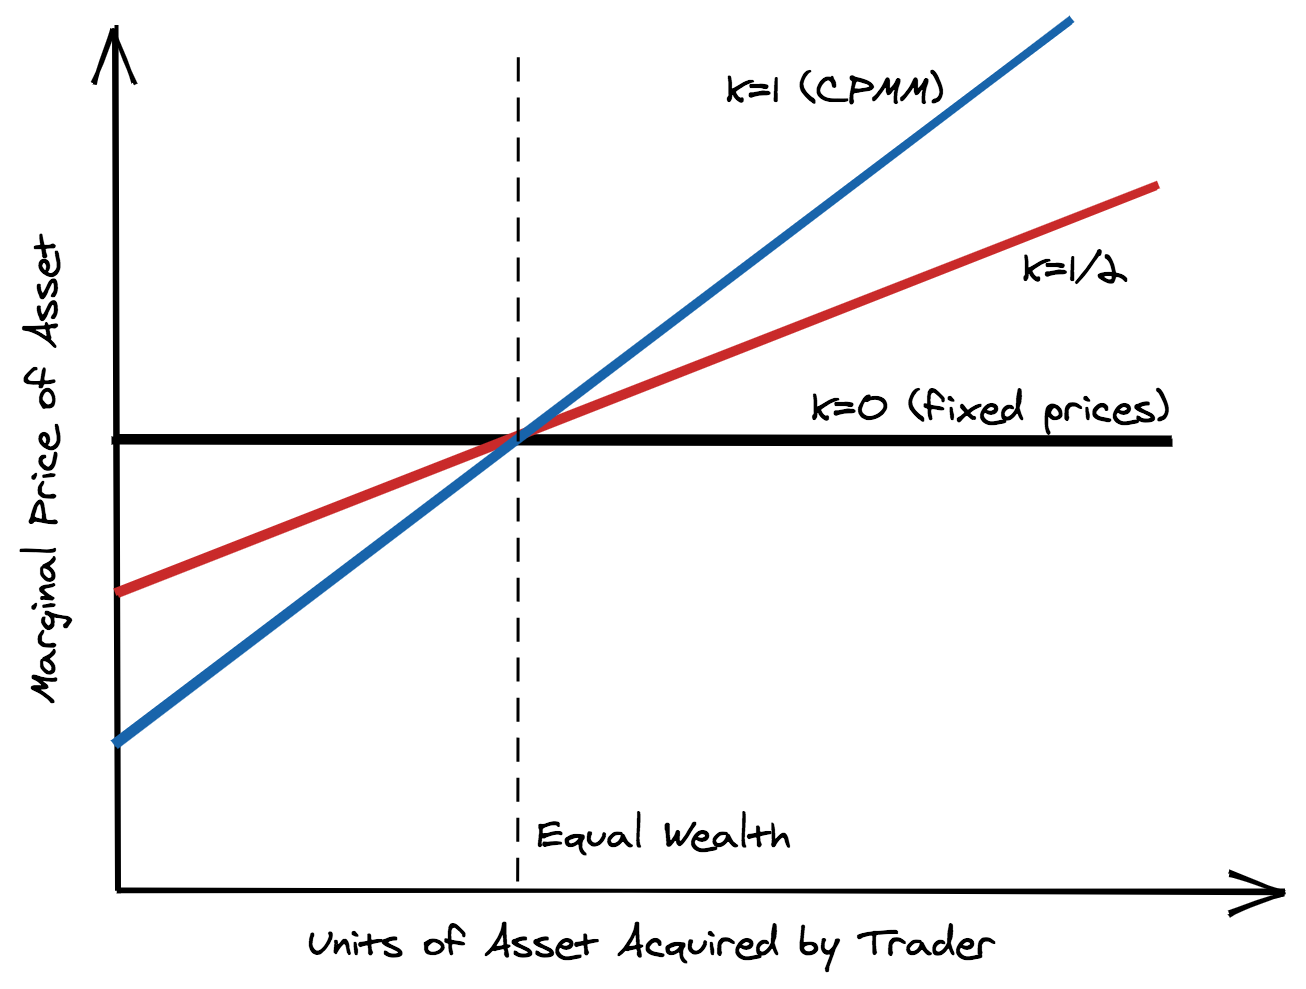
\includegraphics[width=0.66\textwidth]{AssetsAcquired}
\caption{Stylized graphical depiction of slippage within our family of market makers parameterized by $k \in [0,1]$ for an asset that the market maker is currently oversupplied in. The $x$ axis shows the amount of that asset acquired by the trader and the $y$ axis shows the marginal price of the asset from the automated market maker. Because our family of market makers are \emph{price aligned}, the price response curves for all of our invariants will intersect at the point where the market maker has given enough of its oversupplied asset to have equal wealth on every asset (represented here by the dashed vertical line).
}
\label{fig:assetsacquired}
\end{center}
\end{figure}


\begin{table}[htbp]
\begin{center}
\begin{tabular}{|c|c|c|c|c|c|}
\hline
Percent of asset wealth traded &  10\% & 1\% & 0.1\% & 0.01\% & 0.001\% \\
\hline
$k=0$ (fixed prices) & 0 & 0 & 0 & 0 & 0 \\
$k=0.1$ & 101 & 10 & 1.0 & 0.1 & 0.0 \\
$k=0.25$ & 257 & 25 & 2.5 & 0.3 & 0.0 \\
$k=0.5$ & 527 & 50 & 5.0 & 0.5 & 0.1 \\
$k=0.75$ & 811 & 76 & 7.5 & 0.8 & 0.1 \\
$k=0.9$ & 989 & 91 & 9.0 & 0.9 & 0.1 \\
$k=1$ (CPMM) & 1111 & 101 & 10.0 & 1.0 & 0.1 \\
\hline
\end{tabular}
\caption{Price slippage in basis points vs. fixed prices for the invariants with different $k$ parameters when wealths are equal in each asset. To first order, prices slip proportional to both the $k$ parameter and the fraction of wealth traded.}

\end{center}
\label{tab:slipps}
\end{table}%



Since the invariant function is positive homogeneous, the market maker's transactions are positive homogeneous as well. Any transaction with an invariant-based automated market maker can be scaled up or down by a positive multiple as long as the market maker's holdings are also scaled by that same multiple.

This homogeneity suggests that it is meaningful to speak about slippage for transactions expressed as a fraction of the market maker's assets. Table~\ref{tab:slipps} displays the slippage (in basis points) for various transaction sizes and $k$ parameters when the market maker has equal wealth in each asset.

\section{Conclusion}

Automated market makers, such as the constant-product market maker (CPMM) used in Uniswap, are popular in DEXs because maintaining a traditional order book is too expensive on the Ethereum blockchain.
%
The most popular existing DEXs either operate using the prior-free CPMM in two (Uniswap) or three (Balancer) assets, or a fixed price market maker that only uses the market maker's prior value (e.g., 1inch's PMM). 

In this paper we generalized these concepts by introducing a parameterized family of $n$-asset invariants. Our new family spans between the $n$-asset generalization of the CPMM and an $n$-asset fixed-price market maker. The intermediate members of the family represent new and different ways of balancing the market maker's competing goals of risk aversion and profit seeking.

\clearpage

\bibliography{crypto}

\end{document}
